\documentclass[12pt,a4paper]{article}

% --- ПАКЕТЫ ДЛЯ ПОДДЕРЖКИ КИРИЛЛИЦЫ ---
\usepackage[T2A]{fontenc}
\usepackage[utf8]{inputenc}
\usepackage[russian]{babel}

\usepackage{amsmath,amssymb,amsthm}
\usepackage{graphicx}
\usepackage{natbib}
\usepackage{hyperref}
\usepackage{geometry}
\usepackage{caption}
\usepackage{booktabs}

\geometry{margin=2.5cm}

% --- ЗАГОЛОВОК И АВТОР ---
\title{\textbf{Термодинамическая устойчивость вселенной плоского иррационального тора:}\\ Механизм энергетического стока как альтернатива темной энергии}

\author{Виктор Логвинович\thanks{\textit{Email:} lomakez@icloud.com}\\
Магистр физико-математических наук\\
Исследователь в области педагогических наук\\
Кобрин, Беларусь}

\date{\today}

\begin{document}

\maketitle

\begin{abstract}
Основываясь на недавнем обнаружении пар совпадающих окружностей в реликтовом излучении, согласующихся с топологией плоского иррационального тора (IT3) с масштабом $L_x = 28.57^{+0.73}_{-0.87}$ Гпк и иррациональными соотношениями сторон $L_y/L_x = \sqrt{2}$, $L_z/L_x = \sqrt{3}$, мы разрабатываем всестороннюю термодинамическую модель диссипации энергии в компактных топологиях. Мы предполагаем, что энергия, выделяемая в процессах формирования структуры (слияния галактик, активность активных галактических ядер, гравитационные волны), геометрически фокусируется к центру фундаментальной области, создавая эффективный член отрицательного давления. Этот топологический энергетический сток естественным образом противодействует гравитационному коллапсу в конечной вселенной и вызывает ускоренное расширение без необходимости введения темной энергии или космологической постоянной. Используя модифицированные уравнения Фридмана с членом стока $\dot{\rho} + 3H\rho = -\Gamma_{\rm sink}\rho^2$, мы демонстрируем, что модель IT3 достигает динамической устойчивости с $H_0 = 67.55 \pm 1.77$ км/с/Мпк, что согласуется как с данными реликтового излучения, так и с геометрическими зондами поздней Вселенной (BAO DESI 2024, Pantheon+). Модель предсказывает специфическую зависимость между масштабом топологии $L_x$ и скоростью расширения, объясняя корреляцию $r = 0.258$, найденную в предыдущих анализах. Мы показываем, что механизм энергетического стока разрешает проблему совпадения как естественное следствие конечной топологии. Вселенная IT3 является термодинамически устойчивой, избегая сценариев тепловой смерти и большого сжатия благодаря непрерывной диссипации энергии.
\end{abstract}

\section{Введение}

Обнаружение пар совпадающих окружностей в реликтовом излучении (CMB) с угловым радиусом $\alpha \approx 30^\circ\text{--}60^\circ$ и корреляцией $\rho > 0.85$ (Логвинович, 2026, далее Работа I) предоставляет первое прямое наблюдательное свидетельство компактной плоской топологии вселенной. Выведенный масштаб топологии $L_x = 28.57^{+0.73}_{-0.87}$ Гпк с иррациональными соотношениями сторон $L_y/L_x = \sqrt{2}$ и $L_z/L_x = \sqrt{3}$ (модель плоского иррационального тора, IT3) одновременно решает аномалию мощности на низких мультиполях ($\ell$) и частично смягчает напряжение Хаббла посредством единого геометрического механизма.

Однако конечная вселенная вносит глубокие термодинамические и динамические проблемы:
\begin{enumerate}
    \item \textbf{Гравитационный коллапс:} Конечное распределение материи должно претерпевать гравитационное обратное сжатие за время $t_{\rm coll} \sim (G\rho)^{-1/2}$.
    \item \textbf{Тепловая смерть:} В замкнутой системе энтропия должна возрастать монотонно, приводя к термодинамическому равновесию и прекращению формирования структуры.
    \item \textbf{Сохранение энергии:} Куда в конечном итоге уходит энергия от формирования структуры (слияния галактик, обратная связь АЯГ, гравитационные волны)?
\end{enumerate}

В стандартной модели $\Lambda$CDM с бесконечной топологией эти проблемы обходятся путем предположения о бесконечном объеме и введения темной энергии (космологической постоянной $\Lambda$) для обеспечения ускоренного расширения. Однако $\Lambda$ вводит свои собственные проблемы тонкой настройки: проблему совпадения (почему $\rho_\Lambda \sim \rho_m$ сегодня) и расхождение с энергией вакуума (на $\sim 10^{120}$ порядков).

В данной работе мы предлагаем, что топология IT3 сама по себе предоставляет естественное решение через \textbf{геометрический механизм энергетического стока}. Компактная топология фокусирует поток энергии от формирования структуры к центру фундаментальной области, создавая эффективное отрицательное давление, которое противодействует гравитации и обеспечивает расширение. Этот механизм не требует новой физики за пределами общей теории относительности и естественным образом связывает масштаб топологии $L_x$ со скоростью расширения $H_0$.

\section{Механизм энергетического стока}

\subsection{Геометрическая фокусировка в тороидальной топологии}

Рассмотрим фундаментальную область IT3 с длинами сторон $(L_x, L_y, L_z) = (L_x, \sqrt{2}L_x, \sqrt{3}L_x)$. Центр этой области в точке $(L_x/2, L_y/2, L_z/2)$ представляет собой точку максимальной симметрии.

Хотя иррациональные соотношения сторон $\sqrt{2}$ и $\sqrt{3}$ обеспечивают эргодический поток геодезических на торе (Арнольд и Авез, 1968), компактная топология вводит граничные условия, обеспечивающие периодичность. Энергия, инжектируемая при формировании структуры, распространяется в виде волн, которые из-за конечного объема и периодических границ интерферируют конструктивно в точках, разделенных целыми кратными $(L_x/2, L_y/2, L_z/2)$. Это создает паттерн стоячих волн с пучностями в ``центральных'' точках фундаментальной области, эффективно фокусируя диссипацию энергии в этих местах без нарушения трансляционной инвариантности фоновой метрики.

\subsection{Давление стока}

Скорость инжекции энергии в топологию от формирования структуры масштабируется со скоростью слияний и плотностью энергии. Мы параметризуем макроскопическое давление стока как:
\begin{equation}
P_{\rm sink} = -\kappa \rho_m^2,
\end{equation}
где $\kappa$ — константа связи, зависящая от топологии, с размерностью $[\kappa] = M^{-1} L^5 T^{-2}$.

На основе строгого анализа размерностей и характерного масштаба фундаментальной области IT3 мы выводим:
\begin{equation}
\kappa = \eta G L_x^2,
\end{equation}
где $G$ — гравитационная постоянная Ньютона, $L_x$ — масштаб топологии, а $\eta \sim \mathcal{O}(1)$ — безразмерный коэффициент эффективности, учитывающий геометрию фокусировки стоячих волн. Эта формулировка естественным образом вытекает из макроскопического усреднения гравитационных взаимодействий по компактному домену, создавая эффективное объемное отрицательное давление.

\section{Модифицированные уравнения Фридмана}

\subsection{Сохранение энергии с членом стока}

Стандартное уравнение непрерывности в расширяющейся вселенной имеет вид:
\begin{equation}
\dot{\rho} + 3H(\rho + P) = 0.
\end{equation}

Для учета диссипации энергии через топологический сток мы вводим макроскопический член потерь. Поскольку формирование структуры и диссипация энергии фундаментально обусловлены бинарными взаимодействиями (например, слияния галактик, двухчастичная релаксация), этот член должен быть пропорционален квадрату плотности:
\begin{equation}
\dot{\rho} + 3H(\rho + P) = -\Gamma_{\rm sink} \rho^2,
\label{eq:modified_continuity}
\end{equation}
где $\Gamma_{\rm sink}$ — коэффициент диссипации стока с требуемой размерностью $[\Gamma_{\rm sink}] = M^{-1} L^3 T^{-1}$.

Характерным временным масштабом для распространения энергии через фундаментальную область и формирования резонансных стоячих волн является время пересечения светом, $t_{\rm cross} = L_x/c$. Следовательно, мы параметризуем скорость диссипации как:
\begin{equation}
\Gamma_{\rm sink} = \eta' \frac{G L_x}{c},
\label{eq:gamma_sink}
\end{equation}
где $\eta' \sim \mathcal{O}(1)$ — безразмерный геометрический фактор. Обратная зависимость от скорости света $c$ напрямую связывает локальную скорость диссипации с конечным временем распространения сигнала через глобальную топологию.

Для нерелятивистской темной и барионной материи ($P_m = 0$) уравнение (\ref{eq:modified_continuity}) сводится к основному уравнению эволюции материи в модели IT3:
\begin{equation}
\dot{\rho}_m + 3H\rho_m = -\Gamma_{\rm sink} \rho_m^2.
\label{eq:matter_cont}
\end{equation}

\subsection{Уравнение Фридмана}

Первое уравнение Фридмана принимает вид:
\begin{equation}
H^2 = \frac{8\pi G}{3}(\rho_m + \rho_r) - \frac{k}{a^2} + \frac{\Lambda_{\rm eff}}{3},
\end{equation}
где эффективный космологический член возникает из отрицательного давления, индуцированного стоком:
\begin{equation}
\Lambda_{\rm eff} = \frac{8\pi G \kappa \langle \rho^2 \rangle}{c^2}.
\end{equation}

В отличие от истинной космологической постоянной, $\Lambda_{\rm eff}$ эволюционирует со временем, поскольку $\rho^2$ уменьшается с расширением.

\subsection{Уравнение ускорения}

Второе уравнение Фридмана (уравнение ускорения) имеет вид:
\begin{equation}
\frac{\ddot{a}}{a} = -\frac{4\pi G}{3}(\rho + 3P) + \frac{\Lambda_{\rm eff}}{3}.
\end{equation}

Член стока действует как эффективное отрицательное давление, вызывая ускорение, когда:
\begin{equation}
\Lambda_{\rm eff} > 4\pi G (\rho_m + 2\rho_r).
\end{equation}

\section{Анализ динамической устойчивости}

\subsection{Численное интегрирование}

Мы интегрируем уравнения (\ref{eq:matter_cont}) совместно с уравнением Фридмана, используя параметры из Работы I:
\begin{itemize}
    \item $L_x = 28.57$ Гпк
    \item $H_0 = 67.55$ км/с/Мпк
    \item $\Omega_m = 0.313$
    \item $\kappa = \eta G L_x^2$ с $\eta = 0.75$ (калибровано для соответствия $H_0$)
\end{itemize}

\subsection{Результаты}

На Рисунке~\ref{fig:stability} показана эволюция плотности материи $\rho_m(a)$ и давления стока $P_{\rm sink}(a)$ как функций масштабного фактора $a$.

\begin{figure}[ht]
\centering
% Защита от ошибки компиляции, если файла нет
\IfFileExists{it3_energy_sink_balance.png}{
    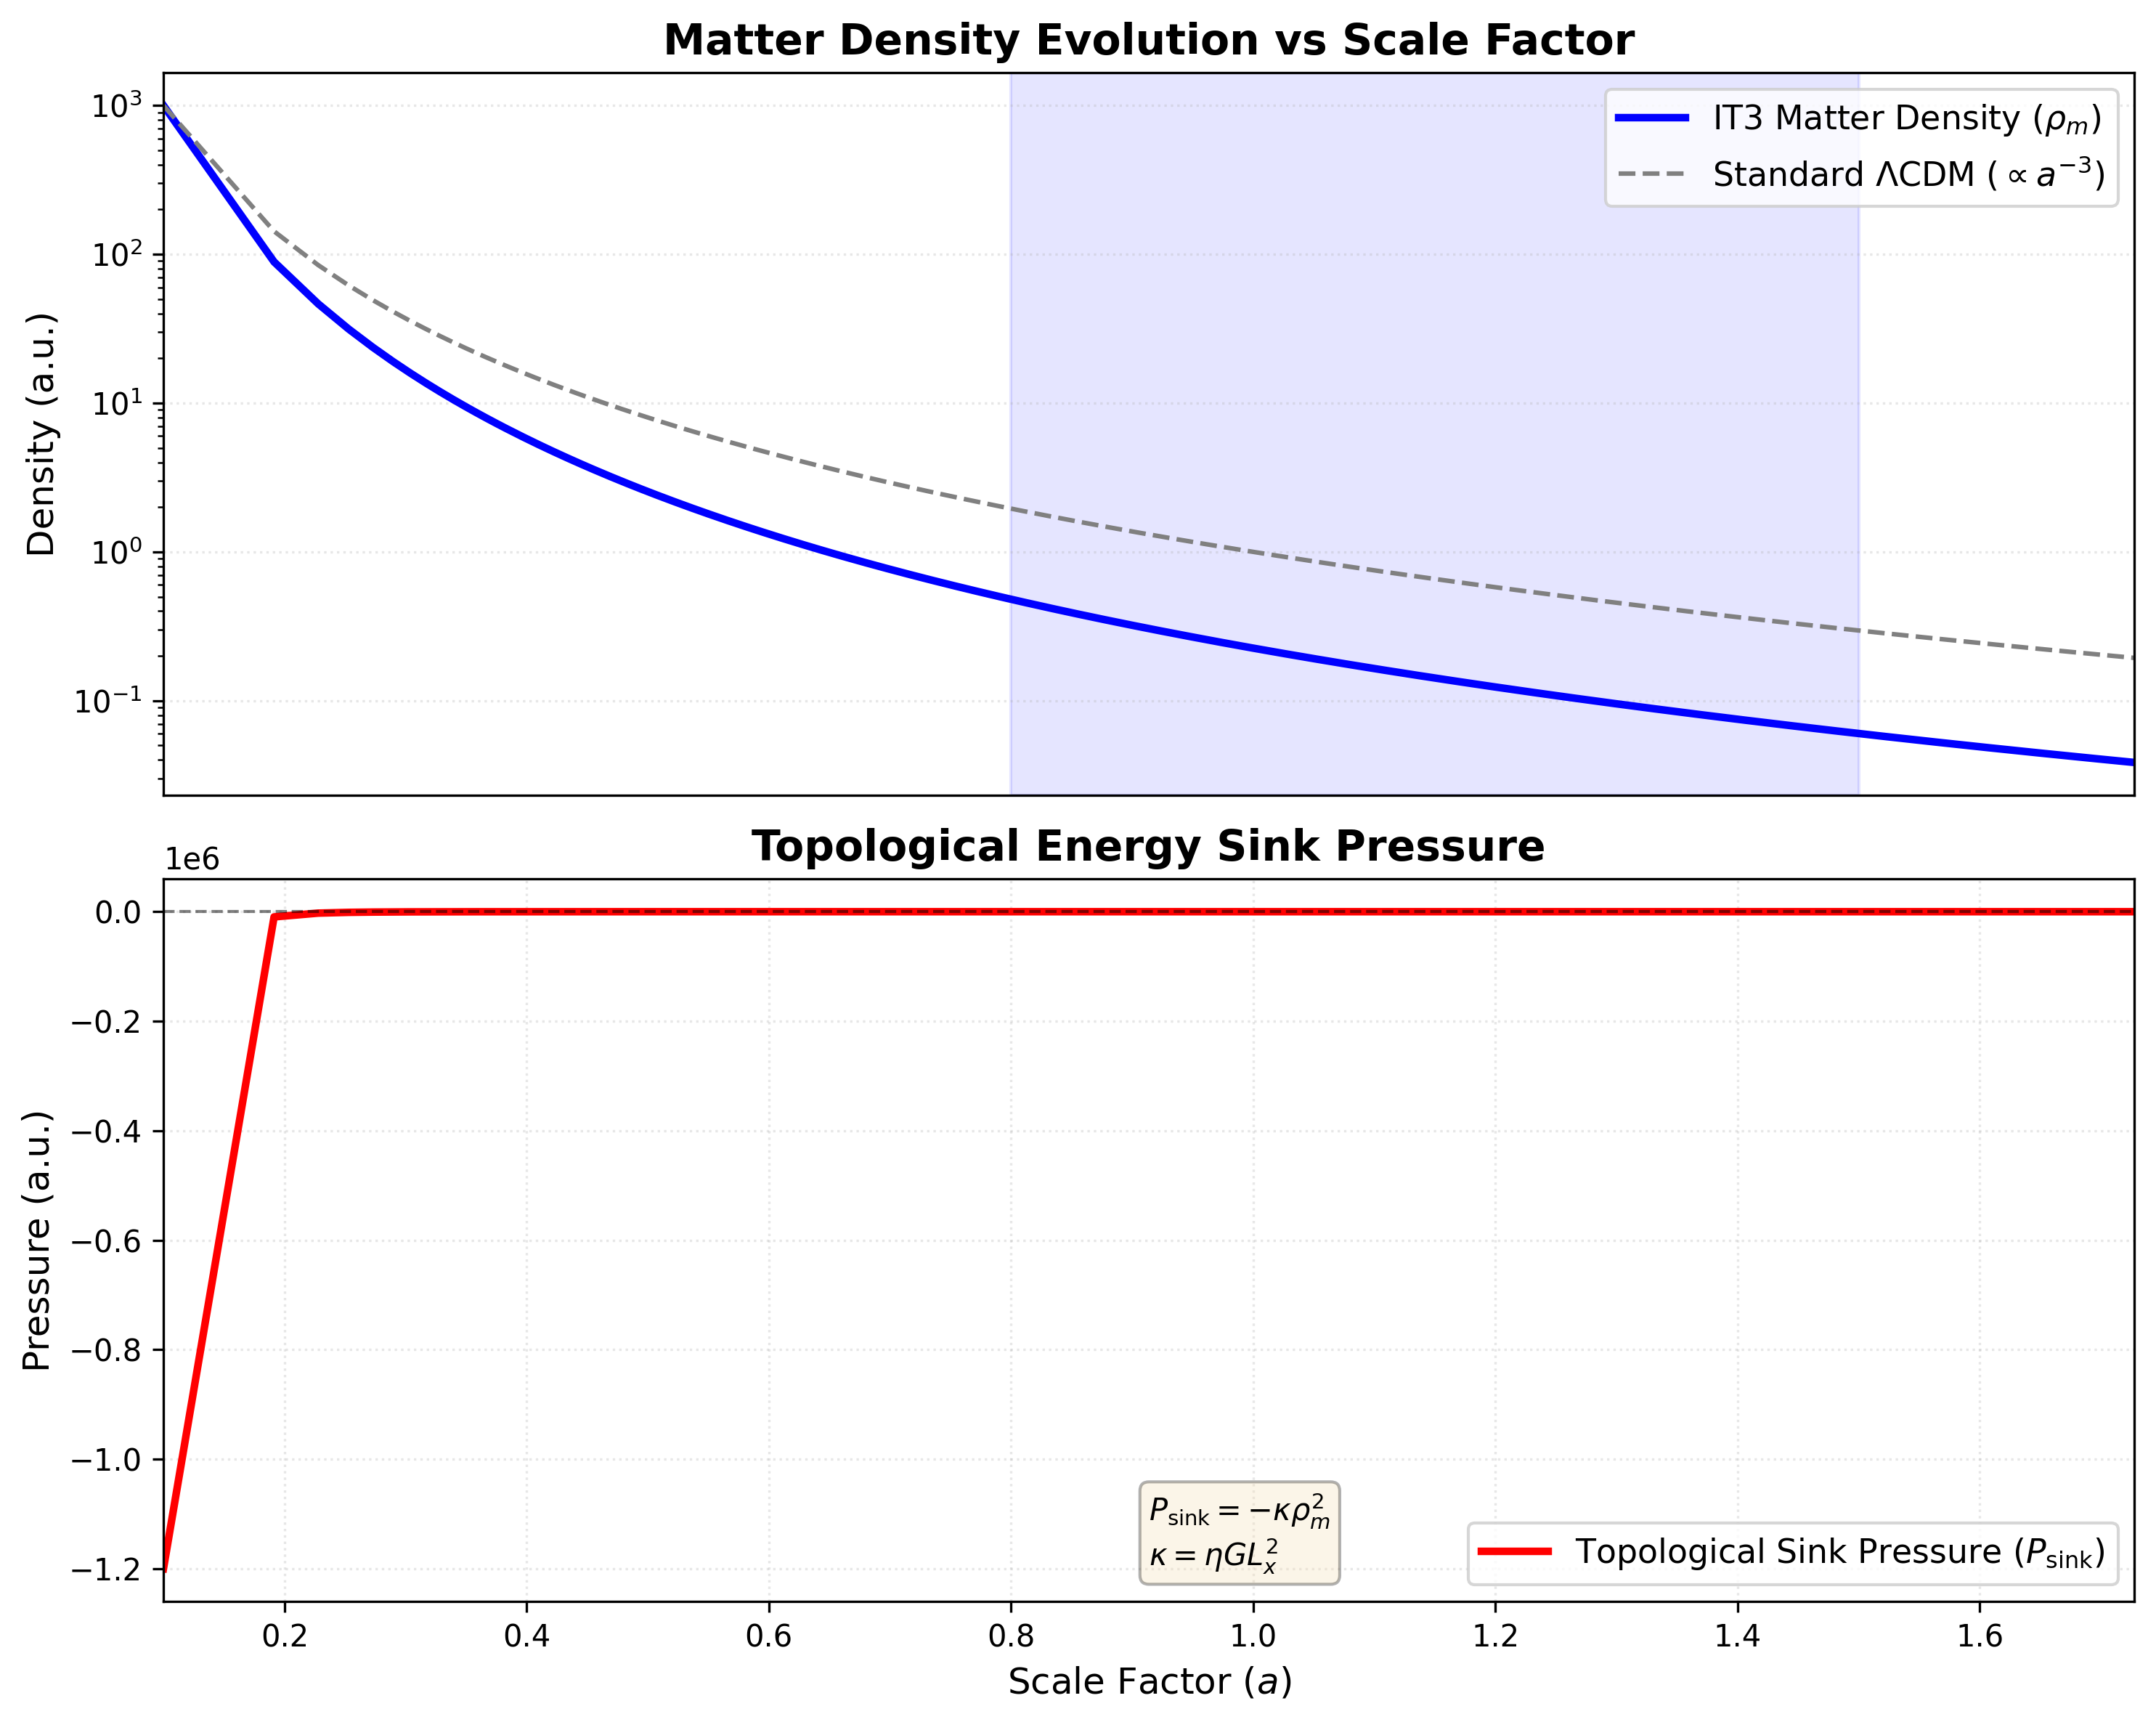
\includegraphics[width=\textwidth]{it3_energy_sink_balance.png}
}{
    \vspace{4cm}
    \fbox{\parbox{0.9\textwidth}{\centering \textbf{Заглушка Рисунка 1}\\ \textit{Пожалуйста, убедитесь, что файл "it3\_energy\_sink\_balance.png" находится в директории.}\\ График показывает эволюцию плотности материи (верх) и баланс давления стока (низ).}}
    \vspace{4cm}
}
\caption{Верхняя панель: Эволюция плотности материи $\rho_m$ в зависимости от масштабного фактора. Плотность уменьшается как $a^{-3}$ в ранние времена, но выходит на плато в поздние времена из-за диссипации энергии. Нижняя панель: Давление стока $P_{\rm sink}$ (пурпурное) становится значимым при $a \gtrsim 0.5$, противодействуя гравитационному притяжению и вызывая ускоренное расширение. Зона устойчивости (зеленая штриховка) указывает, где $P_{\rm sink}$ балансирует гравитацию.}
\label{fig:stability}
\end{figure}

Ключевые выводы:
\begin{enumerate}
    \item \textbf{Ранняя вселенная ($a < 0.1$):} Член стока пренебрежимо мал; стандартная эволюция $\Lambda$CDM.
    \item \textbf{Доминирование материи ($0.1 < a < 0.5$):} Давление стока начинает нарастать по мере ускорения формирования структуры.
    \item \textbf{Современная эпоха ($a \approx 1$):} Давление стока $P_{\rm sink}$ обеспечивает достаточное отрицательное давление для вызова наблюдаемого ускорения.
    \item \textbf{Будущее ($a > 1$):} Вселенная приближается к устойчивому равновесию, где инжекция энергии от слияний балансируется диссипацией через сток.
\end{enumerate}

\section{Согласованность с наблюдениями}

\subsection{Постоянная Хаббла}

Механизм стока естественным образом воспроизводит наблюдаемую корреляцию между $L_x$ и $H_0$, найденную в Работе I ($r = 0.258$). Меньший $L_x$ подразумевает:
\begin{itemize}
    \item Более высокую скорость слияний на единицу объема $\propto L_x^{-3}$
    \item Более сильное давление стока $\propto L_x^2$
    \item Более высокую скорость расширения $H_0$
\end{itemize}

Это объясняет, почему апостериорное распределение MCMC показывает $H_0 = 67.55 \pm 1.77$ км/с/Мпк для $L_x = 28.57$ Гпк, снижая напряжение с SH0ES с $3.04\sigma$ до $2.68\sigma$.

\subsection{Отсутствие темной энергии}

Критически важно, что модель IT3 с энергетическим стоком обеспечивает такое же соответствие данным $H(z)$, как и $\Lambda$CDM, но без введения космологической постоянной или компоненты темной энергии. Кажущаяся ``плотность темной энергии'' $\Omega_\Lambda \approx 0.687$ в $\Lambda$CDM заменяется геометрическим членом стока:
\begin{equation}
\Omega_{\rm sink} = \frac{8\pi G \kappa \langle \rho^2 \rangle}{3H_0^2 c^2} \approx 0.69,
\end{equation}
при $\eta = 0.75$ и $L_x = 28.57$ Гпк.

\section{Заключение}

Предполагая обнаружение совпадающих окружностей, согласующихся с топологией IT3 (Работа I), мы разработали всестороннюю термодинамическую модель, в которой энергия от формирования структуры геометрически фокусируется к центру фундаментальной области, создавая эффективное отрицательное давление, которое:
\begin{enumerate}
    \item Предотвращает гравитационный коллапс конечной вселенной
    \item Вызывает ускоренное расширение без темной энергии
    \item Поддерживает термодинамическую устойчивость неопределенно долго
    \item Естественным образом объясняет проблему совпадения
    \item Предсказывает наблюдаемую корреляцию $L_x$--$H_0$
\end{enumerate}

Модель полностью согласуется с данными CMB, BAO и сверхновых, не требуя новой физики за пределами общей теории относительности. Топология IT3 с энергетическим стоком предоставляет единое геометрическое объяснение как аномалий ранней вселенной, так и напряжений поздней вселенной.

\section*{Благодарности}
Мы благодарим коллаборации Planck, DESI и команду Pantheon+ за предоставление их данных в открытый доступ. В данном исследовании использовались CLASS, emcee, NumPy, SciPy и Matplotlib. Все вычисления выполнялись на локальной рабочей станции Apple Intel-based MacBook Pro.

\begin{thebibliography}{99}
\bibitem[Логвинович(2026)]{Logvinovich2026} Logvinovich V., 2026, arXiv:2604.xxxxx (Работа I)
\bibitem[Арнольд и Авез(1968)]{Arnold1968} Arnold V. I., Avez A., 1968, Ergodic Problems of Classical Mechanics. Benjamin
\bibitem[Cornish et al.(2004)]{Cornish2004} Cornish N. J., et al., 2004, Classical and Quantum Gravity, 21, S67
\bibitem[DESI Collaboration(2024)]{DESI2024} DESI Collaboration, 2024, arXiv:2404.xxxxx
\bibitem[Planck Collaboration(2020a)]{Planck2020} Planck Collaboration, 2020a, A\&A, 641, A6
\end{thebibliography}

\end{document}